%Ultimatives Tool zur Datierung:
%https://www.cc.kyoto-su.ac.jp/~yanom/pancanga/
%skp = ignored in edition
%skm = ignored in xml
\documentclass[10pt]{memoir}
\setstocksize{220mm}{155mm} 	        
\settrimmedsize{220mm}{155mm}{*}	
\settypeblocksize{170mm}{116mm}{*}	
\setlrmargins{18mm}{*}{*}
\setulmargins{*}{*}{1.2}
%\setlength{\headheight}{5pt}%
\checkandfixthelayout[lines]
\linespread{1.16}
\flushbottom

%%% Hyphenation settings
\usepackage[htt]{hyphenat}
\hyphenation{he-lio-trope opos-sum}
\tracingparagraphs=1
%Hyphenation in Devanāgarī of the edition still missing? Probably this needs to be modified in babel-iast package? 

%%% babel
\usepackage[english]{babel}
\usepackage{babel-iast/babel-iast}

\babelfont[iast]{rm}[Renderer=Harfbuzz, Scale=1.3]{AdishilaSan}%AdishilaSan}
\babelfont[english]{rm}{Adobe Text Pro}

%%% more functionality
\PassOptionsToPackage{hyphens}{url}
\usepackage{hyperref}
\usepackage{pdflscape}
\usepackage{cleveref}
\usepackage{url}
\usepackage{cleveref}
\usepackage{microtype}
\usepackage{lineno}

%\usepackage{bigfoot}
%%% more functions
\usepackage[dvipsnames]{xcolor}
%\usepackage[para,perpage]{footmisc}

%%%für den Counter von Kapiteln und Sätzen! 
\newcommand{\uproman}[1]{\uppercase\expandafter{\romannumeral#1}}
\newcommand{\lowroman}[1]{\romannumeral#1\relax}

\makeindex
\newfontfamily\sanskritfont[Script=Devanagari,Mapping=RomDev,Scale=1.1]{Sanskrit2003}
\usepackage{pifont,fourier-orns,lettrine,psvectorian,paralist,enumitem,pdfpages,wrapfig,tabulary,lettrine,longtable}
\setlist[enumerate]{itemsep=0mm}
\usepackage[autostyle]{csquotes}
\usepackage[defaultlines=2,all]{nowidow}
\usepackage{ellipsis,adforn,booktabs,longtable,url,tikz}
\lineskiplimit=-3pt          

\makechapterstyle{IeT}{%
  \chapterstyle{default}
  \renewcommand*{\printchapternonum}{\centering}
  \renewcommand*{\clearforchapter}{\cleartorecto} 
  \aliaspagestyle{chapter}{empty}}
\chapterstyle{IeT}
\setsecnumdepth{none}  \openright  \nouppercaseheads
\settocdepth{subsubsection}

%%%% test better pagebreaks
%\def\fussy{%
%  \emergencystretch\z@
%  \tolerance 200%
%  \hfuzz .1\p@
%  \vfuzz\hfuzz}

%\interfootnotelinepenalty=10000\relax

%\usepackage[maxfloats=256]{morefloats}

%\maxdeadcycles=500

%raggedbottomsectiontrue
%%\checkandfixthelayout


%%%%%%%  biblatex
%\newcommand{\noun}[1]{\textsc{#1}}    %  philosophy-verbose
\usepackage[backend=biber, sorting=nyt, style=verbose]{biblatex} %%%%ORIGINAL TiE
\renewcommand*{\mkbibnamefamily}[1]{\textsc{#1}}


\DeclareFieldFormat{url}{%
  \mkbibacro{URL}\addcolon\space
  \href{#1}{\nolinkurl{\thefield{urlraw}}}}

\DeclareFieldFormat{citeurl}{%
  \href{#1}{\nolinkurl{\thefield{urlraw}}}} 


\DeclareFieldFormat{postnote}{#1}
\renewcommand{\postnotedelim}{, }
\addbibresource{bindu.bib}

%%% ekdosis
\usepackage[teiexport=tidy,parnotes=true]{ekdosis}% =tidy cleans up HTML and XML documents by fixing markup errors and upgrading legacy code to modern standards. parnotes=footnotes below or above critical apparatus

\SetLineation{lineation=page, modulo} %lineation=page sets thenumbering to start afresh at the top of each page. =modulo makes every fifth line numbered. {lineation=page} makes every line numbered! 

\renewcommand{\linenumberfont}{\selectlanguage{english}\footnotesize} %sets language of lines to English

\SetTEIxmlExport{autopar=false} %autopar=falseinstructs ekdosis to ignore blank lines in the.tex sourcefile as markers for paragraph boundaries. As a result, each paragraph of the edition must be found within an environment associated with the xml <p> element

\SetHooks{
  lemmastyle=\bfseries,
  %refnumstyle=\selectlanguage{english}\bfseries,
  refnumstyle=\selectlanguage{english}\color{blue}\bfseries,
  appheight=0.8\textheight,
}

\newif\ifinapparatus
\DeclareApparatus{source}[
%bhook=\inapparatustrue,
lang=english,
notelang=english,
% bhook=\selectlanguage{english},
bhook=\selectlanguage{english}\textbf{Sources:},%
%maxentries=4, 
%ehook=.]
%sep={] },
%nosep,
]

\newif\ifinapparatus
\DeclareApparatus{testium}[
%bhook=\inapparatustrue,
lang=english,
notelang=english,
% bhook=\selectlanguage{english},
bhook=\selectlanguage{english}\textbf{Testimonia:},
%maxentries=4, 
%ehook=.]
%nosep, 
]

% Declare \ifinapparatus and set \inapparatustrue at the beginning of
% the apparatus criticus block. Also set the language.  
\newif\ifinapparatus
  \DeclareApparatus{default}[
  %bhook=\inapparatustrue, 
  lang=english,
  %maxentries=33,
  %bhook=\selectlanguage{english},
  sep = {] },
  delim=\hskip 0.75em,
  rule=\rule{0.7in}{0.4pt},
]

\newif\ifinapparatus
\DeclareApparatus{philcomm}[
%bhook=\inapparatustrue,
lang=english,
notelang=english,
bhook=\selectlanguage{english}\textbf{Philological Commentary:},
%bhook=\selectlanguage{english},
sep={: },
]

\ekdsetup{
showpagebreaks,
spbmk = \textcolor{blue}{spb},
hpbmk = \textcolor{red}{hpb}
}

%\usepackage{fnpos}
%\makeFNmid
%\makeFNbottom
\usepackage[bottom]{footmisc}
%%%%%%%%%%%%%%%%%%%%%%%%%%%
\makeatletter
\def\blfootnote{\gdef\@thefnmark{}\@footnotetext}
\makeatother
%%%%%%%%%%%%%%%%%%%%%%%%%


% Macros and Definitions for the Print of Sigla
\def\acpc#1#2#3{{#1}\rlap{\textrm{\textsuperscript{#3}}}\textsubscript{\textrm{#2}}\space}
\def\sigl#1#2{{{#1}}\textsubscript{\textrm{#2}}}
\def\None{{\sigl{N}{1}}} \def\Noneac{\acpc{N}{1}{ac}\,} \def\Nonepc{\acpc{N}{1}{pc}\,}
\def\Ntwo{{\sigl{N}{2}}} \def\Noneac{\acpc{N}{2}{ac}\,} \def\Nonepc{\acpc{N}{2}{pc}\,}
\def\Done{{\sigl{D}{1}}} \def\Doneac{\acpc{D}{1}{ac}\,} \def\Donepc{\acpc{D}{1}{pc}\,}
\def\Dtwo{{\sigl{D}{2}}} \def\Dtwoac{\acpc{D}{2}{ac}\,} \def\Dtwopc{\acpc{D}{2}{pc}\,}
\def\Uone{{\sigl{U}{1}}} \def\Uoneac{\acpc{U}{1}{ac}\,} \def\Uonepc{\acpc{U}{1}{pc}\,}                 
\def\Utwo{{\sigl{U}{2}}} \def\Utwoac{\acpc{U}{2}{ac}\,} \def\Utwopc{\acpc{U}{2}{pc}\,}

%%%%%%%%%%%%%% Tattvabinduyoga - List of Witnesses   %%%%%%%%%%%%%%%%%%%
\DeclareWitness{ceteri}{\selectlanguage{english}cett.}{ceteri}[]   
\DeclareWitness{E}{\selectlanguage{english}E}{Printed Edition}[]    
\DeclareWitness{P}{\selectlanguage{english}P}{Pune BORI 664}[]  
\DeclareWitness{B}{\selectlanguage{english}B}{Bodleian 485}[]       
\DeclareWitness{N1}{\selectlanguage{english}N\textsubscript{1}}{NGMPP 38/31}[]
\DeclareWitness{N2}{\selectlanguage{english}N\textsubscript{2}}{NGMPP B 38/35}[]
\DeclareWitness{L}{\selectlanguage{english}L}{LALCHAND 5876}[]  
\DeclareWitness{D}{\selectlanguage{english}D}{IGNCA 30019}[] 
%\DeclareWitness{D2}{\selectlanguage{english}D\textsubscript{2}}{IGNCA 30020}[]  
\DeclareWitness{U1}{\selectlanguage{english}U\textsubscript{1}}{SORI 1574}[] 
\DeclareWitness{U2}{\selectlanguage{english}U\textsubscript{2}}{SORI 6082}[]
%%%%%%%%%%%%%% Tattvabinduyoga - Groups of Witnesses   %%%%%%%%%%%%%%%%%%%
\DeclareWitness{X}{\selectlanguage{english}\alpha}{Alpha Group: D,N1,N2,U1}[]
\DeclareWitness{Y}{\selectlanguage{english}\beta}{Beta Group: B,E,L,P,U2}[]
%%%%%%%%%%%%% Testimonia
\DeclareWitness{Ysv}{\selectlanguage{english}Ysv}{Yogasvarodaya}[] %%%add infos!  

%%%%%%%%%%%%%%%%%%%%%%%%%%%%%%%%%%%%%%%%%%%
% Macro for Editing Abbrevs.
\def\om{\textrm{\footnotesize \textit{om.}\ }} %prints om. for omitted in apparatus
\def\korr{\textrm{\footnotesize \textit{em.}\ }} %prints em. for emended in apparatus
\def\conj{\textrm{\footnotesize \textit{conj.}\ }} %prints conj. for conjectured in apparatus

% \supplied{text} EDITORIAL ADDITION -> Within \lem oder \rdg
% \surplus{text} EDITORIAL DELETION -> Within \lem oder \rdg
% \sic{text} CRUX
% \gap{text} LACUNAE -> [reason=??, unit=??, quantity=??, extent=??]


%%%%%%%%%%%%%%%%%%%%%%%%%%%%%%%%%%%%%%%%%%% All macros of this list can be used in 
% Macro for Editing Abbrevs.
\def\eyeskip{\textrm{{ab.\,oc. }}}
\def\aberratio{\textrm{{ab.\,oc. }}}
\def\ad{\textrm{{ad}}}
\def\add{\textrm{{add.\ }}}
\def\ann{\textrm{{ann.\ }}}
\def\ante{\textrm{{ante }}} 
\def\post{\textrm{{post }}}
%\def\ceteri{cett.\,}                   
\def\codd{\textrm{{codd.\ }}}

\def\coni{\textrm{{coni.\ }}}
\def\contin{\textrm{{contin.\ }}}
\def\corr{\textrm{{corr.\ }}}
\def\del{\textrm{{del.\ }}}
\def\dub{\textrm{{ dub.\ }}}

\def\expl{\textrm{{explic.\ }}} 
\def\explica t{\textrm{{explic.\ }}}
\def\fol{\textrm{{fol.\ }}}
\def\foll{\textrm{{foll.\ }}}
\def\gloss{\textrm{{glossa ad }}}
\def\ins{\textrm{{ins.\ }}}      
\def\inseruit{\textrm{{ins.\ }}} 
\def\im{{\kern-.7pt\lower-1ex\hbox{\textrm{\tiny{\emph{i.m.}}}\kern0pt}}} %\textrm{\scriptsize{i.m.\ }}}      
\def\inmargine{{\kern-.7pt\lower-.7ex\hbox{\textrm{\tiny{\emph{i.m.}}}\kern0pt}}}%\textrm{\scriptsize{i.m.\ }}}      
\def\intextu{{\kern-.7pt\lower-.95ex\hbox{\textrm{\tiny{\emph{i.t.}}}\kern0pt}}}%\textrm{\scriptsize{i.t.\ }}}           
\def\indist{\textrm{{indis.\ }}}  
\def\indis{\textrm{{indis.\ }}}
\def\iteravit{\textrm{{iter.\ }}} 
\def\iter{\textrm{{iter.\ }}}
\def\lectio{\textrm{{lect.\ }}}   
\def\lec{\textrm{{lect.\ }}}
\def\leginequit{\textrm{{l.n. }}} 
\def\legn{\textrm{{l.n. }}}
\def\illeg{\textrm{{l.n. }}}

\def\primman{\textrm{{pr.m.}}}
\def\prob{\textrm{{prob.}}}
\def\rep{\textrm{{repetitio }}}
\def\secundamanu{\textrm{\scriptsize{s.m.}}}            \def\secm{{\kern-.6pt\lower-.91ex\hbox{\textrm{\tiny{\emph{s.m.}}}\kern0pt}}}%   \textrm{\scriptsize{s.m.}}}
\def\sequentia{\textrm{{seq.\,inv.\ }}}  
\def\seqinv{\textrm{{seq.\,inv.\ }}}
\def\order{\textrm{{seq.\,inv.\ }}}
\def\supralineam{{\kern-.7pt\lower-.91ex\hbox{\textrm{\tiny{\emph{s.l.}}}\kern0pt}}} %\textrm{\scriptsize{s.l.}}}
\def\interlineam{{\kern-.7pt\lower-.91ex\hbox{\textrm{\tiny{\emph{s.l.}}}\kern0pt}}}   %\textrm{\scriptsize{s.l.}}}
\def\vl{\textrm{v.l.}}   \def\varlec{\textrm{v.l.}} \def\varialectio{\textrm{v.l.}}
\def\vide{\textrm{{cf.\ }}}
\def\cf{\textrm{{cf.\ }}} 
\def\videtur{\textrm{{vid.\,ut}}}
\def\crux{\textup{[\ldots]} }
\def\cruxx{\textup{[\ldots]}}
\def\unm{\textit{unm.}}
%%%%%%%%%%%%%%%%%%%%%%%%%%%%%%%%%%%%

% List of Scholars
\DeclareScholar{ego}{ego}[
forename=Nils Jacob,
surname=Liersch]

% Persons:14\DeclareScholar{ego}{ego}[15forename=Robert,16surname=Alessi]17% Useful shorthands:18\DeclareShorthand{codd}{codd.}{V,I,R,H}19\DeclareShorthand{edd}{edd.}{Lit,Erm,Sm}20\DeclareShorthand{egoscr}{\emph{scripsi}}{ego}

%Useful shorthands:
%\DeclareShorthand{codd}{codd.}{V,I,R,H}
%\DeclareShorthand{edd}{edd.}{Lit,Erm,Sm}
\DeclareShorthand{egoscr}{em.}{ego}
\DeclareShorthand{egoscrconj}{conj.}{ego}
\DeclareShorthand{egomute}{\unskip}{ego}

\usepackage{xparse}

\NewDocumentEnvironment{tlg}{O{}O{}}{\setlength{\leftskip}{0pt}\vspace{-1ex}\begin{quotation}}{\hfill #1\ \vspace{-1ex}\end{quotation}\vspace{-1ex}} %verse environment
%\NewDocumentEnvironment{tlg}{O{}O{}}{\begin{verse}}{॥#1\hskip-4pt ॥\\ \end{verse}}
\NewDocumentCommand{\tl}{m}{{\selectlanguage{iast} #1}}

\NewDocumentCommand{\extra}{m}{{\textcolor{gray}{#1}}} %command for additions to U2
\NewDocumentCommand{\crazy}{m}{{\textcolor{red}{#1}}} %totally corrupted passage
\NewDocumentCommand{\coro}{m}{{\textcolor{violet}{#1}}} %colour for sentence counter! 

\NewDocumentEnvironment{prose}{O{}}{\begin{otherlanguage}{iast}}{\end{otherlanguage}}
% \NewDocumentEnvironment{padd}{O{}}{\begin{otherlanguage}{iast}}{\end{otherlanguage}}
\NewDocumentEnvironment{tlate}{O{}}
%\NewDocumentEnvironment{tadd}{O{}}

%Define two commands: \skp ("sanskrit plus"), to be ignored by TeX in
%the edition text, but processed in the TEI output. Conversely, \skm
%("sanskrit minus") is to be processed in the edition text, but
%ignored if found in the apparatus criticus and in the TEI output:

\NewDocumentCommand{\skp}{m}{}
\TeXtoTEIPat{\skp {#1}}{#1}

%\NewDocumentCommand{\skpp}{m}{}
%\TeXtoTEIPat{\skpp {#1}}{#1}

\NewDocumentCommand{\skm}{m}{\unless\ifinapparatus#1-\fi}
\TeXtoTEIPat{\skm {#1}}{}

% \NewDocumentCommand{\dd}{}{/\hskip-4pt/}
\NewDocumentCommand{\dd}{}{\mbox{/\hskip-4pt/}}
\TeXtoTEIPat{\dd {}}{//}


%%% modify environments and commands
%%% TEI mapping
\TeXtoTEIPat{\begin {tlg}}{<lg>} %lg=(Group of verse (s)) contains one or more verses or lines of verse that together form a formal unit (e.g. stanza, chorus).
\TeXtoTEIPat{\end {tlg}}{</lg>}

\TeXtoTEIPat{\begin {prose}}{<p>}
\TeXtoTEIPat{\end {prose}}{</p>}

\TeXtoTEIPat{\begin {tlate}}{<p>}
\TeXtoTEIPat{\end {tlate}}{</p>}

\TeXtoTEIPat{\\}{}
\TeXtoTEIPat{\linebreak}{<br/>}
\TeXtoTEIPat{\noindent}{}
%\TeXtoTEI{tl}{l}
\TeXtoTEI{emph}{hi}
\TeXtoTEI{bigskip}{}
\TeXtoTEI{None}{N1}
\TeXtoTEI{Ntwo}{N2}
\TeXtoTEI{Done}{D1}
\TeXtoTEI{Dtwo}{D2}
\TeXtoTEI{Uone}{U1}
\TeXtoTEI{Utwo}{U2}
%\TeXtoTEIPat{/}{ |}
%\TeXtoTEI{//}{ ||}
\TeXtoTEIPat{\korr}{em. }
\TeXtoTEIPat{\conj}{conj.}
\TeXtoTEIPat{\om}{om.}
\TeXtoTEIPat{english}{}
\TeXtoTEIPat{\hskip}{}
\TeXtoTEIPat{\hskip-4pt}{}
\TeXtoTEIPat{\hskip-2pt}{}
\TeXtoTEIPat{-}{ }
\TeXtoTEIPat{4pt}{}
\TeXtoTEIPat{2pt}{}
\TeXtoTEIPat{\textcolor {#1}{#2}}{<hi rend="#1">#2</hi>} 

% Nullify \selectlanguage in TEI as it has been used in
% \DeclareWitness but should be ignored in TEI.
\TeXtoTEI{selectlanguage}{}



\FormatDiv{1}{\begin{center}\Large}{\end{center}}
\FormatDiv{2}{\begin{center}\small}{\end{center}}
\FormatDiv{3}{\bfseries}{.}
\title{Tattvayogabindu of Rāmacandra\\ A Critical Edition and Annotated Translation\\ and a Comparative Analysis of the \\Complex Early Modern Yoga Yaxonomies }
\date{\today}
\parindent=15pt

\begin{document}

\frontmatter
\thispagestyle{empty} % Verhindert Seitenzahl auf der Seite
\begin{center}

%\vspace{0.5in}

%\begin{otherlanguage}{iast}
%   \large\sanskritfont{Tattvayogabindu}\\
%\end{otherlanguage}

\vspace{0.25in}


\huge\textbf{\MakeUppercase{The Tattvayogabindu \\of Rāmacandra}}\\

\vspace{0.2in}

\Large  Critical Edition and Annotated Translation of an Early Modern Text on Rājayoga, with a Comparative Analysis of the Complex Yoga Taxonomies from the Same Period\\ 

\vspace{0.45in}

\thispagestyle{empty}
\end{center}
%\newpage
%\thispagestyle{empty}
%\mbox{}
%\newpage

\newpage

  \thispagestyle{empty}
  \begin{figure}[p]
    \centering
    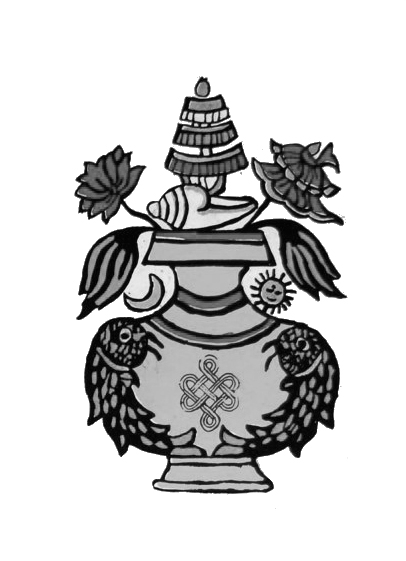
\includegraphics[width=0.25\textwidth]{pics/purna.jpg}
  \end{figure}
  
\newpage

\begin{landscape}
\thispagestyle{empty}
  \begin{figure}[p]
	\centering
  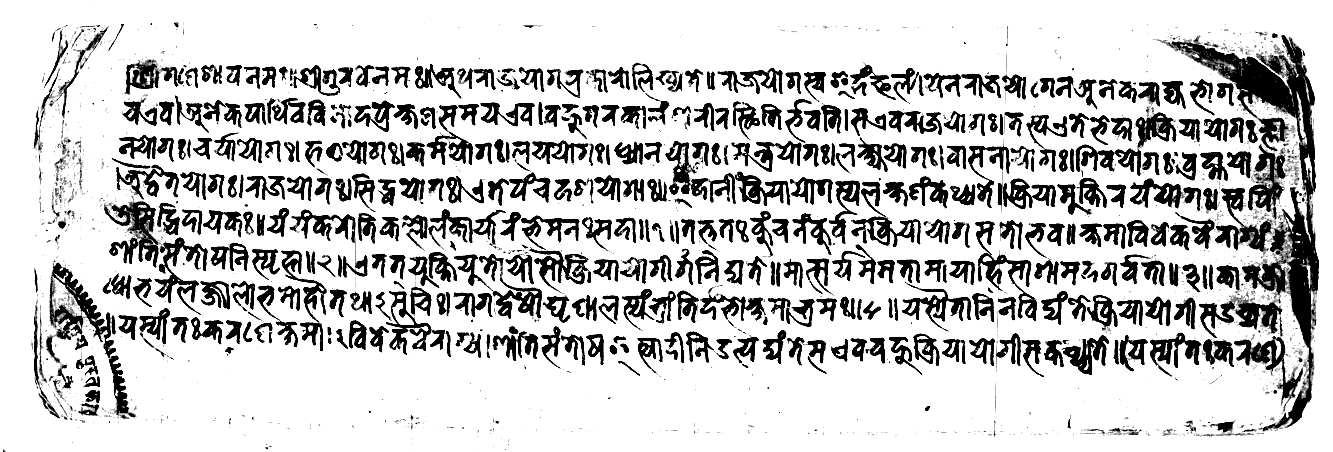
\includegraphics[width=1.5\textwidth]{pics/folio1.jpg}
	\caption{Folio 1v of Ms. \getsiglum{N1}.}
	 \phantomsection\label{fig_folio1}
\end{figure}
\end{landscape}

\cleardoublepage
\tableofcontents
\thispagestyle{empty}
\newpage 
\listoffigures
\thispagestyle{empty}
\newpage
\listoftables
\thispagestyle{empty}
\newpage

\mainmatter
\pagestyle{defaultstyle}
\counterwithout{footnote}{chapter}
\counterwithout{figure}{chapter}
\counterwithout{table}{chapter}
\renewcommand{\thetable}{\arabic{table}}
%%%tables 
\setsecnumdepth{section}
\maxsecnumdepth{subsubsection}
\newpage
\chapter{Introduction}
\cleardoublepage

\section{General remarks}
 \phantomsection\label{generalremarks}
 \lettrine{T}{he} \textit{Tattvayogabindu} of Rāmacandra\footnote{A discussion about the author Rāmacandra is found on p. \pageref{ramarama}.} is an early modern Sanskrit text on Rājayoga that was written in the first half of the seventeenth century\footnote{The dating of the text is discussed on p. \pageref{dating}.} in northern India.\footnote{The detailed discussion of the place of origin is found on p. \pageref{riversrivers}, n. \ref{riversrivers}.} The most salient feature of the work that makes it historically significant is its highly differentiated taxonomy of types of yoga.\footnote{This is a remarkable increase in the number of declared yogas compared to the standard medieval tetrad of Mantra, Laya, Haṭha and Rājayoga.} In the \textit{Tattvayogabindu}'s introduction, most manuscripts name fifteen types of yoga, presented as methods of Rājayoga. These are 1. Kriyāyoga, 2. Jñānayoga, 3. Caryāyoga, 4. Haṭhayoga, 5. Karmayoga, 6. Layayoga, 7. Dhyānayoga, 8. Mantrayoga, 9. Lakṣyayoga, 10. Vāsanāyoga, 11. Śivayoga, 12. Brahmayoga, 13. Advaitayoga, 14. Siddhayoga, and 15. Rājayoga itself. The text is a yogic compendium written in a mix of mainly prose and 47 verses in textbook-style, where its 59 topics are introduced in sections most of the time launched by recognizable phrases. The sections deal with the methods of Rājayoga and their effects, but others also cover topics like yogic physiology, the Avadhūta, the importance of the guru, cosmogony, and a \textit{yogaśāstrarahasya}.  

The \textit{Tattvayogabindu} has not been discussed comprehensively or considered in the secondary literature on yoga. The only exception is \citeauthor{birch2014} (2014: 415–416) who briefly described its list of fifteen yogas in the context of the ``fifteen medieval yogas'' and noted that a similar taxonomy occurs in Nārāyaṇatīrtha’s \textit{Yogasiddhāntacandrikā} (17th century), a commentary on the \textit{Pātañjalayogaśāstra} that integrates fifteen medieval yogas within its \textit{aṣṭāṅga} format. An incomplete account of the fifteen yogas is found within the Sanskrit yoga text \textit{Yogasvarodaya}, which is known only through quotations in the \textit{Prāṇatoṣinī}, the \textit{Yogakarṇikā} and the \emph{Śabdakalpadruma}.\footnote{Manuscripts under the name of \textit{Yogasvarodaya} seem to be lost. I was not able to locate the manuscripts of the text in any manuscript catalogue at hand.} The \textit{Yogasvarodaya} announces a total of fifteen yogas but names only eight of them in its introductory \textit{śloka}s. It is the primary source and template for the compilation of the \textit{Tattvayogabindu}. Besides several passages, Rāmacandra, in many instances, follows its content and structure by rewriting the \textit{Yogasvarodaya}’s \textit{śloka}s into prose or quoting them directly without attribution. Due to the incomplete transmission of the \textit{Yogasvarodaya}, Rāmacandra’s \textit{Tattvayogabindu} is a natural and valuable starting point for an unprecedented in-depth study of the complex early modern yoga taxonomies, a phenomenon that can be narrowed down precisely in terms of time and as I will show regarding its localisation. The other source text that Rāmacandra used is the \textit{Siddhasiddhāntapaddhati} whose content he draws on, particularly in the second half of his composition. Another text that includes an almost similar taxonomy of twelve yogas divided into three tetrads\footnote{See p.\pageref{sarvasarva} for a detailed discussion of the \textit{Sarvāṅgayogapradīpikā}.} is Sundardās’s \textit{Brajbhāṣā} yoga text named \textit{Sarvāṅgayogapradīpikā} which not just shares most of the types of yogas but also provides a different and valuable perspective on the addressed yoga categories.\footnote{For a comparative table of the complex early modern yoga taxonomies see table \ref{tab:complextaxonomies} on p. \pageref{tab:complextaxonomies}.}

These complex taxonomies that emerged during the 17th century crossed sectarian divides and were adapted to the specific needs of different authors and traditions. The \textit{Tattvayogabindu} thus encapsulates a large proportion of the diversity of yoga types and teachings after the \textit{Haṭhapradīpikā} (15th century) that were adopted and practised by a broad spectrum of religious traditions and strata of Indian society. In the particular case of the \textit{Tattvayogabindu}, there are various statements throughout the text that reveal a strategy to detach yoga from its ascetic and renunciate connotations and to stylise Rājayoga as a practice that can bring the desired soteriological benefits even to practitioners who enjoy worldly pleasures and expensive lifestyles. Textual evidence suggests that the \textit{Tattvayogabindu} is an important example of a text that provides an early modern adaptation of Rājayoga for \textit{kṣatriya}s in a courtly environment.

One printed edition of the \textit{Tattvayogabindu} was published in 1905 with a Hindi translation and based on (an) unknown manuscript(s).\footnote{\emph{Binduyoga}. \textit{Binduyogaḥ with Bhāṣaṭīkā}. Ed. by Jvālāprasāda Miśra. Mumbai, 1905.} This publication has the title ``\textit{Binduyoga}'' confirmed by the printed text’s colophon. However, as I will discuss in the introduction, the text was originally known as \textit{Tattvayogabindu}. The consulted manuscripts contain significant discrepancies, structural differences and variant readings between them and the printed edition.\footnote{For example, the printed edition does not contain the complex yoga taxonomy presented in the manuscripts of the \emph{Tattvayogabindu}.} Furthermore, the manuscripts are scattered over the northern half of the Indian subcontinent and Nepal, which suggests that the text was widely transmitted at some point. Lengthy passages of the \textit{Tattvayogabindu} are quoted without attribution in a text called \textit{Yogasaṃgraha} and Sundaradeva’s \textit{Haṭhasaṅketacandrikā}.

The first chapter of this dissertation contains a general introduction to Rāmacandra's \textit{Tattvayogabindu}. The chapter gives a brief overview of the content of the text and discusses its origin, the author and the author's intended audience. Subsequently, the textual witnesses, source texts and testimonies of the \textit{Tattvayogabindu} are described. A stemmatic analysis of the text is then presented, based on manual philological observation and computer-assisted stemmatics to present a \textit{stemma codicum}. The chapter concludes with a presentation of the editorial policies, which form the basis for the second chapter of this thesis.
The second chapter, the core of this dissertation, is a critical edition and annotated translation of the \textit{Tattvayogabindu}. The critical edition significantly improves the text and sheds new light on its historical significance.
The third chapter contains a comparative analysis of the complex early modern yoga taxonomies based on hermeneutics of difference.\footnote{The conceptof hermeneutics of difference is discussed on p. \pageref{hermeneutics}, n. \ref{hemerneutics}.}  Using the new critical edition of the \textit{Tattvayogabindu} and the texts mentioned above, \emph{Yogasvarodaya}, \emph{Yogasiddhāntacandrikā} and \emph{Sarvāṅgayogapradīpikā}, the complex yogic taxonomies of the four texts are compared in detail. Based on this comparative analysis, a differentiated hypothesis on the emergence of the complex yoga taxonomies was developed, and the complex yoga taxonomies were located und explained in the broader context of the historical development of the yoga traditions. The comparison includes a nuanced description of each yoga category used by the authors of the texts with complex yoga taxonomies. While the authors of the four texts often operate with identical terms for the individual yoga categories, they interpret these categories according to their religious backgrounds and agendas, with intriguing and exciting differences. Contrasting the comparanda, i.e. the authors, the texts, the yoga taxonomies and the yoga categories, therefore provides a deep insight into the discursive negotiation processes of the Indian yoga traditions of the 17th century.


\chapter{Conventions in the Critical Apparatus}
\section{Sigla in the Critical Apparatus}

\begin{itemize}
\item \beta : \getsiglum{D}, \getsiglum{J}, \getsiglum{K1}, \getsiglum{N1}, \getsiglum{N2}, \getsiglum{U1}
\item \gamma : \getsiglum{B}, \getsiglum{E}, \getsiglum{L}, \getsiglum{P}, \getsiglum{U2}
\item B : Bodleian Oxford D 4587
\item C : \emph{Haṭhasaṅketacandrikā} GOML Ms. No. R 3239
\item C\textsubscript{pc} : \emph{Haṭhasaṅketacandrikā} GOML Ms. No. R 3239
\item cett.: ceteri (all manuscripts except the ones mentioned in the lemma)
\item \Done : IGNCA 30019
\item E : Printed Edition
\item J : JNUL Ms. No. 55769
\item Jo : \emph{Haṭhasaṅketacandrikā} MMPP MS. No. 2244
\item \Kone : AS G 11019
\item L : Lalchand Research Library LRL5876
\item M : \emph{Haṭhasaṅketacandrikā} ORI Ms. No. B 220
\item \Ntwo : NGMPP B 38-35 / A 1327-14
\item \None : NGMPP B 38-31
\item P : Pune BORI 664
\item PT : \emph{Prāṇatoṣiṇī}
\item \Uone : SORI 1574
\item \Utwo : SORI 6082
\item V : OI MSU 10558
\item YK : \emph{Yogakarṇikā}% 
\item YSv : \emph{Yogasvarodaya}
\end{itemize}
\newpage

\chapter[Critical Edition \& Annotated Translation of the \emph{Tattvayogabindu}]{The \emph{Tattvayogabindu} of Rāmacandra \\ \huge  
  Critical Edition \& Annotated Translation}
\pagestyle{chapter2style}
\newpage
\begin{alignment}[
  texts=edition[class="edition"];
  translation[class="translation"],
  ]
  \begin{edition}
    \ekddiv{
      head={[\uproman{37}. \textbf{piṇḍamadhye saptasamudrāḥ}]},
      type=section,
      depth=2, 
      n=XXXVII
    }
    \xmlhead[h37]{[XXXVII. piṇḍamadhye saptasamudrāḥ]}
    \phantomsection
      \addcontentsline{toc}{section}{XXXVII. piṇḍamadhye saptasamudrāḥ}
    \phantomsection\label{saptasamudra}
       \begin{prose}[p37_01]
      \noindent
%----------------------------
%idānīṃ piṃḍamadhye saptasamudrāḥ kathyante// prasvedamadhye kṣārasamudraḥ/   \E
%idānīṃ piṃḍamadhye saptasamudrāḥ kathyaṃte   prasvedamadhye kṣārasamudraḥ    \P
%idānīṃ piṃḍamadhye samudrāḥ      kathyate//  prasvedamadhye kṣārasamudraḥ//  \B
%idānīṃ piṃḍamadhye samudrāḥ      kathyaṃte// prasvedamadhye sārasasamudraḥ// \L
%\om                                                                          \N1
%idānīṃ piṃḍamadhye saptasamudrāḥ kathyete//  prasvedamadhye kṣārasasamudra   \D
%idānīṃ piṃḍamadhye saptasamudrāḥ kathyaṃte//  prasvedamadhye kṣārasasamudra   \K1
%idānīṃ piṃḍamadhye saptasamudrāḥ kathyaṃte//  prasvedamadhye kṣārasasamudraḥ//   \J      
%\om                                                                          \N2
%idānīṃ piṃḍamadhye saptasamudrāḥ kathyaṃte      svedamadhye kṣārasasamudraḥ  \U1 %%%288.jpg
%idānīṃ piṃḍamadhye saptasamudrāḥ kathyaṃte// prasvedamadhye kṣārasāgaraḥ//   \U2
%-----------------------------
%Now the seven oceans within the body are taught. (1) Within sweat is the salt ocean. 
%----------------------------
      \note[type=source, labelb=_106b, labele=_106e, nosep]{cf. YSv (PT, pp. 842-43): samudrāḥ sapta kathyante piṇḍamadhye vyavasthitāḥ | lavaṇekṣusurāsarpirdadhidugdhajalāntakāḥ | lavaṇaṃ svedamadhye tu ikṣūrakte madhu tvaci | sarpir medo vasāmadhye dadhi kṣīraṃ lalāṭake | vīryamadhye 'mṛto jñeyaḥ pāde kūrmaḥ sthito mahān |}
      \note[type=source, labelb=_106b, labele=_106e, nosep]{cf. SSP 3.8 (Ed. p. 29): mūrte kṣārasamudraḥ | śukre 'mṛtasamudraḥ | lālāyāṃ kṣīrasamudraḥ | kaphe dadhisamudraḥ | medasi ghṛtasamudraḥ | vasāyāṃ madhusamudraḥ | rakte ikṣusamudraḥ | evaṃ saptasamudrāḥ ||}
idānīṃ piṇḍamadhye\linelabel{_106b}
\app{\lem[wit={ceteri}]{saptasamudrāḥ}
  \rdg[wit={B,L}]{samudrāḥ}}\hfill
\app{\lem[wit={ceteri}]{kathyante}
  \rdg[wit={B}]{kathyate}
  \rdg[wit={D}]{kathyete}}/\hfill
\app{\lem[wit={ceteri}]{prasvedamadhye}
  \rdg[wit={U1}]{svedamadhye}}\hfill
\app{\lem[wit={ceteri}]{kṣārasamudraḥ}
  \rdg[wit={L}]{sārasasamudraḥ}
  \rdg[wit={U1}]{kṣārasasamudraḥ}
  \rdg[wit={K1}]{kṣārasasamudra}
  \rdg[wit={U2}]{kṣārasāgaraḥ}}\dd{}\hfill
%----------------------------
%lalāṭamadhye kṣīraḥ samudraḥ/            vāṅmadhye                                 madhusamudraḥ/  kaphamadhye  dadhisamudraḥ/  medomadhye ghṛtasamudraḥ/  \E
%lālāmadhye   kṣīrasamudraḥ               vasāmadhye                                madhusamudraḥ   kaphamadhye  dadhisamudraḥ   medomadhye ghṛtasamudraḥ   \P
%lalāṭamadhye kṣīrasamudraḥ// raktamadhye vasāmadhye                                madasamudraḥ    kaphamadhye  dadhisamudraḥ// medomadhye ghṛtasamudraḥ// \B
%lalāṭamadhye kṣīrasamudraḥ// raktamadhye vasāmadhye                                madyasamudraḥ// kaphamadhye  dadhisamudraḥ// medamadhye ghṛtasamudraḥ// \L
%\om                                                                 \N1
%lalāṭamadhye kṣīrasamudraḥ/              vasāmadhye                                                             dadhisamudraḥ// medamadhye ghṛtasamudraḥ// \D
%lalāṭamadhye kṣīrasamudraḥ/              vasāmadhye                                                             dadhisamudraḥ// medamadhye ghṛtasamudraḥ// \K1
%lalāṭamadhye kṣīrasamudraḥ//              vasāmadhye                                                             dadhisamudraḥ// medamadhye ghṛtasamudraḥ// \J
%\om                                                                                                                                                         \N2
%lalāṭamadhye kṣīrasamudraḥ               vasāmadhye                                                             dadhisamudraḥ   medamadhye ghṛtasamudraḥ   \U1 %%%288.jpg
%lalāṭamadhye kṣīrasamudraḥ//             vīryamadhye svāduḥ samudraḥ// majjāmadhye madhusamūdraḥ// kaphamadhye  dadhisamudraḥ// medamadhye ghṛtasamudraḥ// \U2
%-----------------------------
%(2) Within the forehead is the milk ocean. (3) Within the marrow is the honey-ocean. (4) In the phlegm is the sour milk ocean. (5) In the fat is the butter ocean.  
%----------------------------
\app{\lem[wit={ceteri}]{lalāṭamadhye}
  \rdg[wit={P}]{lālāmadhye}}\\
\app{\lem[wit={ceteri}, alt={kṣīrasamudraḥ}]{kṣīrasamudraḥ}
  \rdg[wit={E}]{kṣīraḥ samudraḥ}}\dd{}
\app{\lem[wit={ceteri},alt={vasāmadhye}]{vasāmadhye}
  \rdg[wit={E}]{vāṅmadhye}
  \rdg[wit={U2}]{vīryamadhye svāduḥ samudraḥ || majjāmadhye}}
\app{\lem[wit={E,P}]{madhusamudraḥ}
  \rdg[wit={B}]{madasamudraḥ}
  \rdg[wit={L}]{madyasamudraḥ}
  \rdg[wit={U2}]{madhusamūdraḥ}
  \rdg[wit={D,J,K1,U1}]{\om}}\dd{}
\app{\lem[wit={ceteri}]{kaphamadhye}
  \rdg[wit={D,J,K1,U1}]{\om}} dadhisamudraḥ\dd{}
\app{\lem[wit={B,E,P}, alt={medo°}]{medo}
 \rdg[wit={ceteri}]{meda°}}madhye ghṛtasamudraḥ\dd{}
%----------------------------
%                           rasamadhye   ikṣurasasamudraḥ// vīryamadhye svādusamudraḥ/                pādamadhye kūrmasthānam//   \E
%                           raktamadhye  ikṣurasasamudraḥ   vīryamadhye svādudakasamudraḥ             pādamadhye kūrmasthānam     \P
%                                        ikṣusamudraḥ/      vīryamadhye svādukasamudraḥ/  karmasthāna pādasamadhye/               \B
%                                        ikṣusamudraḥ//     vīryamadhye svādukasamudraḥ// karmasthāna pādamadhye                  \L
%\om                                                                                                                             \N1
%vasāmadhye madhusamudraḥ// raktamadhye  ikṣusamudraḥ//     vīryamadhye amṛtasamudraḥ/                pādam tale  kūrmasthānaṃ/    \D
%vasāmadhye madhusamudraḥ// raktamadhye  ikṣusamudraḥ//     vīryamadhye amṛtasamudraḥ//                pādam tale  kūrmasthānaṃ/  \K1
%npāmadhye madhusamudraḥ// raktamadhye  ikṣusamudraḥ//     vīryamadhye mṛtasamudraḥ//cha//           pādamadhye  kūrmasthānaṃ/    \J
%\om                                                                                                                             \N2
%vasāmadhye madhusamudraḥ   raktamadhye  ikṣurasamudraḥ     vīryamadhye mṛtasamudraḥ                  pādamadhye kūrmasthānaṃ     \U1 %%%288.jpg
%                           raktamadhye  ikṣurasamudraḥ//                                                                         \U2
%-----------------------------
% (6) Within the blood is the sugar ocean. (7) Within the semen is the ocean of the nectar of immortality. Situated at [their] feet is the place of the turtle. 
%----------------------------
\app{\lem[wit={P,U1,U2}]{raktamadhye}
  \rdg[wit={D,U1}]{vasāmadhye madhusamudraḥ || raktamadhye}
  \rdg[wit={J}]{npāmadhye madhusamudraḥ || raktamadhye}
  \rdg[wit={E}]{rasamadhye}}
\app{\lem[wit={ceteri}]{ikṣusamudraḥ}
  \rdg[wit={U1,U2}]{ikṣurasamudraḥ}
  \rdg[wit={E,P}]{ikṣurasasamudraḥ}}\dd{}
%\note[type=philcomm, labelb=278, lem={ikṣura°}]{Due to \textit{sandhi} \textit{akṣura°} would be exspected, but was probably misregarded for clarity.}
vīryamadhye\app{\lem[wit={J,U1}]{'mṛtasamudraḥ}
  \rdg[wit={D,K1}]{amṛtasamudraḥ}
  \rdg[wit={E}]{svādusamudraḥ}
  \rdg[wit={B,L}]{svādukasamudraḥ}
  \rdg[wit={P}]{svādudakasamudraḥ}}\dd{}
\app{\lem[wit={ceteri}]{pādamadhye}
  \rdg[wit={B}]{karmasthāna pādasamadhye}
  \rdg[wit={L}]{karmasthāna pādamadhye}
  \rdg[wit={D,K1}]{pādam tale}}
\app{\lem[wit={ceteri}]{kūrmasthānam}
  \rdg[wit={D,J,K1,U1}]{kūrmastānaṃ}
  \rdg[wit={B,L}]{\om}}\dd{}\linelabel{_106e}
\end{prose}
  \end{edition}
  \begin{translation}
    \ekddiv{
      head={[\uproman{37}. \textbf{Seven oceans within the body}]},
      type=section,
      depth=2, 
      n=XXXVII.1
    }
    \xmlhead[h37]{[XXXVII. Seven oeans within the body]}
    \begin{tlate}[p37_01]
     \noindent
Now, the seven oceans within the body are taught.\footnote{Rāmacandra, who bases his descriptions of the seven oceans on the YSv (PT, pp. 842-43) (cf. sources on the previous page) changed the order of oceans sightly. The respective passage can be translated as follows: ``The seven oceans are taught to be situated within the body, [one of each] containing salt (\textit{lavaṇa}), sugar (\textit{ikṣu}), wine (\textit{surā}), butter (\textit{sarpir}), sour milk (\textit{dadhi}), milk (\textit{dugdha}) and water (\textit{jala}). (1) Salt is within the sweat, (2) sugar in the blood, (3) wine in the skin, (4) ghee in the fat, (5-6) sour milk and milk in the forehead. (7) The nectar of immortality is known to be situated within the semen. A big turtle* (*the earth imagined as a tortoise floating on water) is situated at their feet.''} (1) Within the sweat is the salt ocean. (2) Within the forehead is the milk ocean. (3) Within the marrow is the honey ocean. (4) In the phlegm is the sour milk ocean. (5) In the fat is the ghee ocean. (6) Within the blood is the sugarcane ocean. (7) Within the semen is the ocean of the nectar of immortality. Situated at the feet is the place of the turtle.\footnote{The earth consisting of seven islands with mount meru in its centre represented as a tortoise floating on waters of the seven oceans, cf. \citetitle{markandeya} 58, \citetitle{bhagavata} 5.16-26 and \citeauthor[2009: 354]{bryant2009}.}
\flushpage
\end{tlate}
  \end{translation}
\end{alignment}
\pagebreak %after pp. 115-116
%%%%%%%%%%%%%%%%%%%%%%%%%%%%%%%%%%%%%%%%%%
%%%%%%%%%%%%%%%%%%%%%%%%%%%%%%%%%%%%%%%%%% 
%%%%%%%%PAGEBREAK%%%%%%%PAGEBREAK%%%%%%%%%
%%%%%%%%%%%%%%%%%%%%%%%%%%%%%%%%%%%%%%%%%% 
%%%%%%%%%%%%%%%%PAGEBREAK%%%%%%%%%%%%%%%%%
%%%%%%%%%%%%%%%%%%%%%%%%%%%%%%%%%%%%%%%%%% 
%%%%%%%%PAGEBREAK%%%%%%%PAGEBREAK%%%%%%%%%
%%%%%%%%%%%%%%%%%%%%%%%%%%%%%%%%%%%%%%%%%% 
%%%%%%%%%%%%%%%%%%%%%%%%%%%%%%%%%%%%%%%%%% 
%%%%%%%%%%%%%%%%%%%%%%%%%%%%%%%%%%%%%%%%%% 
%%%%%%%%%%%%%%%%%%%%%%%%%%%%%%%%%%%%%%%%%% 
%%%%%%%%PAGEBREAK%%%%%%%PAGEBREAK%%%%%%%%%
%%%%%%%%%%%%%%%%%%%%%%%%%%%%%%%%%%%%%%%%%% 
%%%%%%%%%%%%%%%%PAGEBREAK%%%%%%%%%%%%%%%%%
%%%%%%%%%%%%%%%%%%%%%%%%%%%%%%%%%%%%%%%%%% 
%%%%%%%%PAGEBREAK%%%%%%%PAGEBREAK%%%%%%%%%
%%%%%%%%%%%%%%%%%%%%%%%%%%%%%%%%%%%%%%%%%% 
%%%%%%%%%%%%%%%%%%%%%%%%%%%%%%%%%%%%%%%%%% 
%%%%%%%%%%%%%%%%%%%%%%%%%%%%%%%%%%%%%%%%%% 
%%%%%%%%%%%%%%%%%%%%%%%%%%%%%%%%%%%%%%%%%% 
%%%%%%%%PAGEBREAK%%%%%%%PAGEBREAK%%%%%%%%%
%%%%%%%%%%%%%%%%%%%%%%%%%%%%%%%%%%%%%%%%%% 
%%%%%%%%%%%%%%%%PAGEBREAK%%%%%%%%%%%%%%%%%
%%%%%%%%%%%%%%%%%%%%%%%%%%%%%%%%%%%%%%%%%% 
%%%%%%%%PAGEBREAK%%%%%%%PAGEBREAK%%%%%%%%%
%%%%%%%%%%%%%%%%%%%%%%%%%%%%%%%%%%%%%%%%%% 
%%%%%%%%%%%%%%%%%%%%%%%%%%%%%%%%%%%%%%%%%% 
 \begin{alignment}[
  texts=edition[class="edition"];
  translation[class="translation"],
  ]
  \begin{edition}
\ekddiv{
  head={[\uproman{38}. \textbf{navadvāramadhye navakhaṇḍāni}]},
  type=section,
  depth=2, 
  n=XXXVIII
}
\xmlhead[h38]{[XXXVIII. navadvāramadhye navakhaṇḍāni]}
\phantomsection
\addcontentsline{toc}{section}{XXXVIII. navadvāramadhye navakhaṇḍāni}
\phantomsection\label{ninecontinents}
    \begin{prose}[p38_01]
      \noindent
%----------------------------      
%idānīṃ navadvāreṣu                                                                                 nāsikayoḥ kinnarakhaṃḍanaraharikhaṃḍauḥ netrayoḥ ketumāla bhadrāśvau/ karṇayoḥ hiraṇmayakhaṃḍa ramyakakhaṃḍau/ gude kurukhaṃḍaḥ   liṃge ilāvṛtakhaṇḍaḥ// \E  [p.51]
%idānīṃ navadvāreṣu     navakhaṃjani? kathyaṃte                              mukhe bharatakhaṃḍaḥ 1 nāsikayoḥ kinarakhaṃḍe 3                netrayoḥ ketumāla bhadrāśve 4 karṇayor hiraṇmayaramyaka khaṃdaḥ 5      gude kurukhaṃḍaḥ 6 liṃge ilāvṛtaḥ 7  \P 7659.jpg!!!
%idānīṃ                 navakhaṃḍāni  kathyaṃte/                             mukhe bharatakhaṃḍaḥ   nāsikayor madhye kināraharikhaṃḍā/      netrayo ketumāla bhadrāsve/   karṇayor hiraṇyamayaramyakhaṃḍaḥ/        gude kurukhaṃḍāḥ/  liṃge iḍṛttaṃ??/ \B DSCN7169.JPG Z.4
%idānīṃ                 navakhaṃḍāni  kathyaṃte//                            mukhe bharatakhaṃḍaḥ// nāsikayor madhye kinārasiṃhakhaṃḍā      netrayo ketumāla bhadrāsve//   karṇayor hiraṇyamayaramyakhaṃḍaḥ        gude kurukhaṃḍāḥ//  liṃge ilāvṛtaṃ// \L   0025.jpg
%\om                                                                 \N1
%idānīṃ navadvāramadhye navakhaṃḍāḥ   kathyaṃte//                                  bharatakhaṃḍaḥ/ kāśmīrakhaṃḍaḥ/ strīmaṃḍalakhaṃḍaḥ/     dvijakhaṃḍaḥ/ ekapādakhaṃḍaḥ/  rākṣasakhaṃḍaḥ  gāṃdhārakhaṃḍaḥ// kaivarttakhaṃḍaḥ// garbhakhaṃḍaḥ// \D %%%p.14 verso
%idānīṃ navadvāramadhye navakhaṃḍāḥ   kathyaṃte//                                  bharatakhaṃḍaḥ/ kāśmīrakhaṃḍaḥ/ strīmaṃḍalakhaṃḍaḥ/     dvijakhaṃḍaḥ// ekapādakhaṃḍaḥ//  rākṣasakhaṃḍaḥ  ghāṃdhārakhaṃḍaḥ// kaivarttakhaṃḍaḥ// garbhakhaṃḍaḥ// \K1
%idānīṃ navadvāramadhye navakhaṃḍāḥ   kathyaṃte//                                  bharatakhaṃḍaḥ// kāśmīrakhaṃḍaḥ// strīmaṃḍalakhaṃḍaḥ//     dvijakhaṃḍaḥ// ekapādakhaṃḍaḥ//  rākṣasakhaṃḍaḥ//  gāṃdhārakhaṃḍaḥ// kaivarttakhaṃḍaḥ// garbhakhaṃḍaḥ//cha// \J      
%\om                                                                 \N2
%idānīṃ navadvāramadhye navakhaṃḍāḥ   kathyate                                     bharatakhaṃḍaḥ  kāsmīrakhaṃḍaḥ strīmaṃḍalakhaṃḍaḥ   ???dvīttakhaṃḍaḥ yekapādakhaṃḍaḥ rākṣasakhaṃḍaḥ gaṃdhārakhaṃḍaḥ  kaivartakhaṃḍaḥ   garbhakaṃḍhaḥ \U1
%idānīṃ navadvāreṣu     navakhaṃḍāṇi  kathyaṃte// pādamadhye kūrmasthānaṃ// mukhaṃ bhāratakhaṃḍaṃ// nāsikayoḥ// kinnara// harikhaṃḍa//       netrayoḥ// ketumāla// bhadraśve karṇayoḥ// hiraṇmaya// ramyakakaṃḍe// gude kurukhaṃḍaṃ// liṃge ulāvṛtaṃ// evaṃ navakhaṃḍāḥ//    \U2
%-----------------------------
%Now, the nine continents within the nine doors are taught: Bharata (1), Kaśmīra (2), Strīmaṃḍala (3), Dvija (4), Ekapāda (5), Rākṣasa (6), Ghandhāra (7), Kaivartta (8) [and] Garbha (9). 
%----------------------------
\note[type=source, labelb=_107b, labele=_107e, nosep]{cf. YSv (PT, p. 843): idānīn tu navadvāre navakhaṇḍāni saṃśṛṇu | pāyvādau bhārataṃ khaṇḍaṃ kāśmīraṃ trikamaṇḍalam | dvijakhaṇḍam ekapādaṃ khaṇḍaṃ vakṣye samaṇḍalam | kaivarttaṃ garttagāndhāraṃ navakhaṇḍam iti sthitam |}
\note[type=source, labelb=_107b, labele=_107e, nosep]{cf. SSP 3.9 (Ed. p. 55): navakhaṇḍāḥ nava dvāreṣu vasanti| bhāratakhaṇḍaḥ kāśmīrakhaṇḍaḥ karparakhaṇḍaḥ śrīkhaṇḍaḥ śaṅkhakhaṇḍaḥ ekapādakhaṇḍaḥ gāndhārakhaṇḍaḥ kaivartakhaṇḍaḥ mahāmerukhaṇḍaḥ evaṃ navakhaṇḍāḥ |}
%\note[type=philcomm, labelb=280, lem={\uproman{38}\textsuperscript{\lowroman{1}-\lowroman{2}}}]{There is complete divergence between the two main groups of manuscripts. I edited according to the \beta-group, since their readings are very close to the source texts.}% These are the well-known nine \textit{dvīpa}s or islands ruled by nine sons of Ṛṣabhadeva, which are the nine \textit{varṣa}s of Jambudvīpa, viz., Bhārata, Kinnara, Hari, Kuru, Hiraṇmaya, Ramyaka, Ilāvṛta, Bhadrāśva and Ketumāla.}
idānīṃ\linelabel{_107b}
\app{\lem[wit={D,E,J,K1,U1}]{navadvāramadhye}
  \rdg[wit={E,P,U2}]{navadvāreṣu}
  \rdg[wit={B,L}]{\om}}\hfill
\app{\lem[wit={B,P,L,U2}]{navakhaṇḍāni}
  \rdg[wit={D,J,K1,U1}]{navakhaṃḍāḥ}
  \rdg[wit={E}]{\om}}\hfill
\app{\lem[wit={ceteri}]{kathyante}
  \rdg[wit={U1}]{kathyate}}/\hfill
\app{\lem[wit={D,J,K1,U1}]{bharatakhaṇḍaḥ}
  \rdg[wit={B,P,L}]{mukhe bharatakhaṃḍaḥ}
  \rdg[wit={U2}]{pādamadhye kūrmasthānaṃ || mukhaṃ bhāratakhaṃḍaṃ}
  \rdg[wit={E}]{\om}}\dd{}\hfill
\app{\lem[wit={D,J,K1,U1}]{kāśmīrakhaṃḍaḥ}
  \rdg[wit={E}]{nāsikayoḥ kinnarakhaṃḍanaraharikhaṃḍauḥ}
  \rdg[wit={P}]{nāsikayoḥ kinarakhaṃḍe 3}
  \rdg[wit={B}]{nāsikayor madhye kināraharikhaṃḍā}
  \rdg[wit={L}]{nāsikayor madhye kinārasiṃhakhaṃḍā}
  \rdg[wit={U2}]{nāsikayoḥ || kinnara || harikhaṃḍa}}\dd{}\hfill
\app{\lem[wit={D,J,K1,U1}, alt={strīmaṇḍalakhaṇḍaḥ}]{strī:\\maṇḍalakhaṇḍaḥ}
  \rdg[wit={ceteri}]{\om}}\dd{}\hfill
\app{\lem[wit={D,J,K1,U1}]{dvijakhaṇḍaḥ}
  \rdg[wit={E}]{netrayoḥ ketumāla bhadrāśvau}
  \rdg[wit={P}]{netrayoḥ ketumāla bhadrāśve 4}
  \rdg[wit={B,L}]{netrayo ketumāla bhadrāsve}
  \rdg[wit={U2}]{netrayoḥ || ketumāla || bhadraśve}}\dd{}\hfill
\app{\lem[wit={D,J,K1}]{ekapādakhaṇḍaḥ}
  \rdg[wit={U1}]{yekapādakhaṃḍaḥ}
  \rdg[wit={ceteri}]{\om}}\dd{}\hfill
\app{\lem[wit={D,J,K1,U1}]{rākṣasakhaṇḍaḥ}
  \rdg[wit={E}]{karṇayoḥ hiraṇmayakhaṃḍa ramyakakhaṃḍau}
  \rdg[wit={P}]{karṇayor hiraṇmayaramyakakhaṃdaḥ 5}
  \rdg[wit={B,L}]{karṇayor hiraṇyamayaramyakhaṃḍaḥ}
  \rdg[wit={U2}]{karṇayoḥ || hiraṇmaya || ramyakakaṃḍe}}\dd{}\hfill
\app{\lem[wit={D,J,K1}]{gāndhārakhaṇḍaḥ}
  \rdg[wit={U1}]{gaṃdhārakhaṇḍaḥ}
  \rdg[wit={E}]{gude kurukhaṃḍaḥ}
  \rdg[wit={P}]{gude kurukhaṃḍaḥ 6}
  \rdg[wit={B,L}]{gude kurukhaṃḍāḥ}
  \rdg[wit={U2}]{gudekurukhaṃḍaṃ}}\dd{}\\
\app{\lem[wit={D,J,K1,U1}, alt={kaivarttakhaṇḍaḥ}]{kaivarttakhaṇḍaḥ}
  \rdg[wit={E}]{liṃge ilāvṛtakhaṇḍaḥ}
  \rdg[wit={P}]{liṃge ilāvṛtaḥ 7}
  \rdg[wit={B,L}]{ilāvṛtaṃ}
  \rdg[wit={U2}]{liṃge ulāvṛtaṃ}}\dd{}
\app{\lem[wit={D,K1,U1}]{garbhakhaṇḍaḥ}
  \rdg[wit={J}]{garbhakhaṇḍaḥ || cha ||}
  \rdg[wit={U2}]{evaṃ navakhaṃḍāḥ}
  \rdg[wit={ceteri}]{\om}}\dd{}\linelabel{_107e}%\vspace*{\fill}
\end{prose}
  \end{edition}
  \begin{translation}
\ekddiv{
  head={[\uproman{38}. \textbf{Nine regions within the nine Doors}]},
  type=section,
  depth=2, 
  n=XXXVIII.1
}
\xmlhead[h38]{[XXXVIII. Nine regions within the nine Doors]}
\begin{tlate}[p38_01] \noindent
  Now, the nine continents\footnote{The island of Jambudvīpa consists of nine continents.} within the nine orifices\footnote{The nine doors (\textit{navadvāra}) refer to the nine openings of the body: mouth, nostrils, eyes, ears, anus and gender.} are taught: Bharata (1), Kāśmīra (2), Strīmaṇḍala (3), Dvija (4), Ekapāda (5), Rākṣasa (6), Gāndhāra (7), Kaivartta (8) [and] Garbha (9).\footnote{There is a complete divergence between the two main groups of manuscripts. I have edited according to the \beta-group, since its readings are much closer to the source texts. A thoughtful scribe of the \gamma-group must have been dissatisfied with the original nomenclature and the supposedly original absence of the names of the nine doors in his exemplar, and therefore felt compelled to rewrite the passage. Consequently, the \gamma-group transmits this section with an alternative nomenclature for the nine regions and includes the complete set of the names of the nine doors. These names are partially preserved in the \citetitle{ramatosana} and entirely absent from the \citetitle{ssplonavla}. The \gamma-group locates (1) the Bharatakhaṇḍa within the mouth, (2–3) the Kinnara- and Harikhaṇḍa in the two nostrils, (4–5) the Ketumāla- and Bhadrāśva[-khaṇḍa] in the eyes, (6–7) the Hiraṇyamaya- and Ramyaka[-khaṇḍa] in the ears, (8) the Kurukhaṇḍa at the anus, and (9) the Ilāvṛta[-khaṇḍa] at the genitals. This system, along with a detailed and elaborate description, is presented in \citetitle{parakhya} 5.61–93.}
  \flushpage
  \end{tlate}
  \end{translation}
\end{alignment}
\pagebreak %after pp. 117-118
\cleardoublepage
\selectlanguage{english}
\chapter{Appendix}
\section{Figures}
 
% \begin{landscape}
\clearpage

  \begin{figure}[ht]
	\centering
  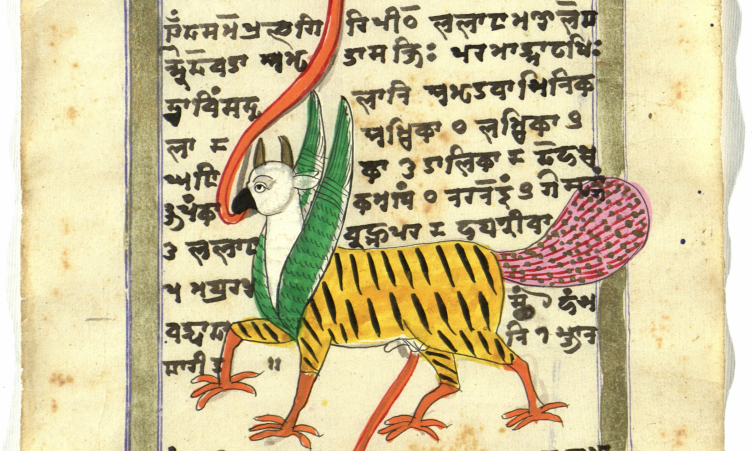
\includegraphics[width=1\textwidth]{pics/Wolpertinger.png}
\caption[The \textit{dehasvarūpa} of \textit{ajapāgāyatrī}]{The \textit{dehasvarūpa} of \textit{ajapāgāyatrī}. The image, reminiscent of a hippogriff, is part of an illustrated Sanskrit manuscript written in the Śāradā script. Preserved as a single large scroll under Acc. No. 1334 at the Oriental Institute in Srinagar (Kashmir), it is entitled \textit{Nāḍīcakra}. The manuscript contains a depiction of the yogic body’s \textit{cakra}s and \textit{nāḍī}s. The text surrounding the figure closely corresponds to the additional material found in manuscript \getsiglum{U2} of the \textit{Tattvayogabindu}. The manuscript reads (diplomatic transcription): \textit{oṃ daśame pūrṇagiripīṭhe lalāṭamaṇḍale candro devatā amṛtāśaktiḥ paramātmā ṛṣiḥ dvāviṃśaddalāni amṛtavāsinikalā 4: ambikā 1 lambikā 2 gha(ṃ)ṭkā 3 tālikā 4 dehasvarūpaṃ kākamukhaṃ 1 naranetraṃ 2 gośṛṅgaṃ 3 lalāṭabrahmapara 4 hayagrīvā 5 mayūramuśchaṃ 6 haṃsacārītani 7 sthāna.}}
	\phantomsection\label{fig_wolpertinger}
      \end{figure}

      \clearpage

  \begin{figure}[ht]
	\centering
  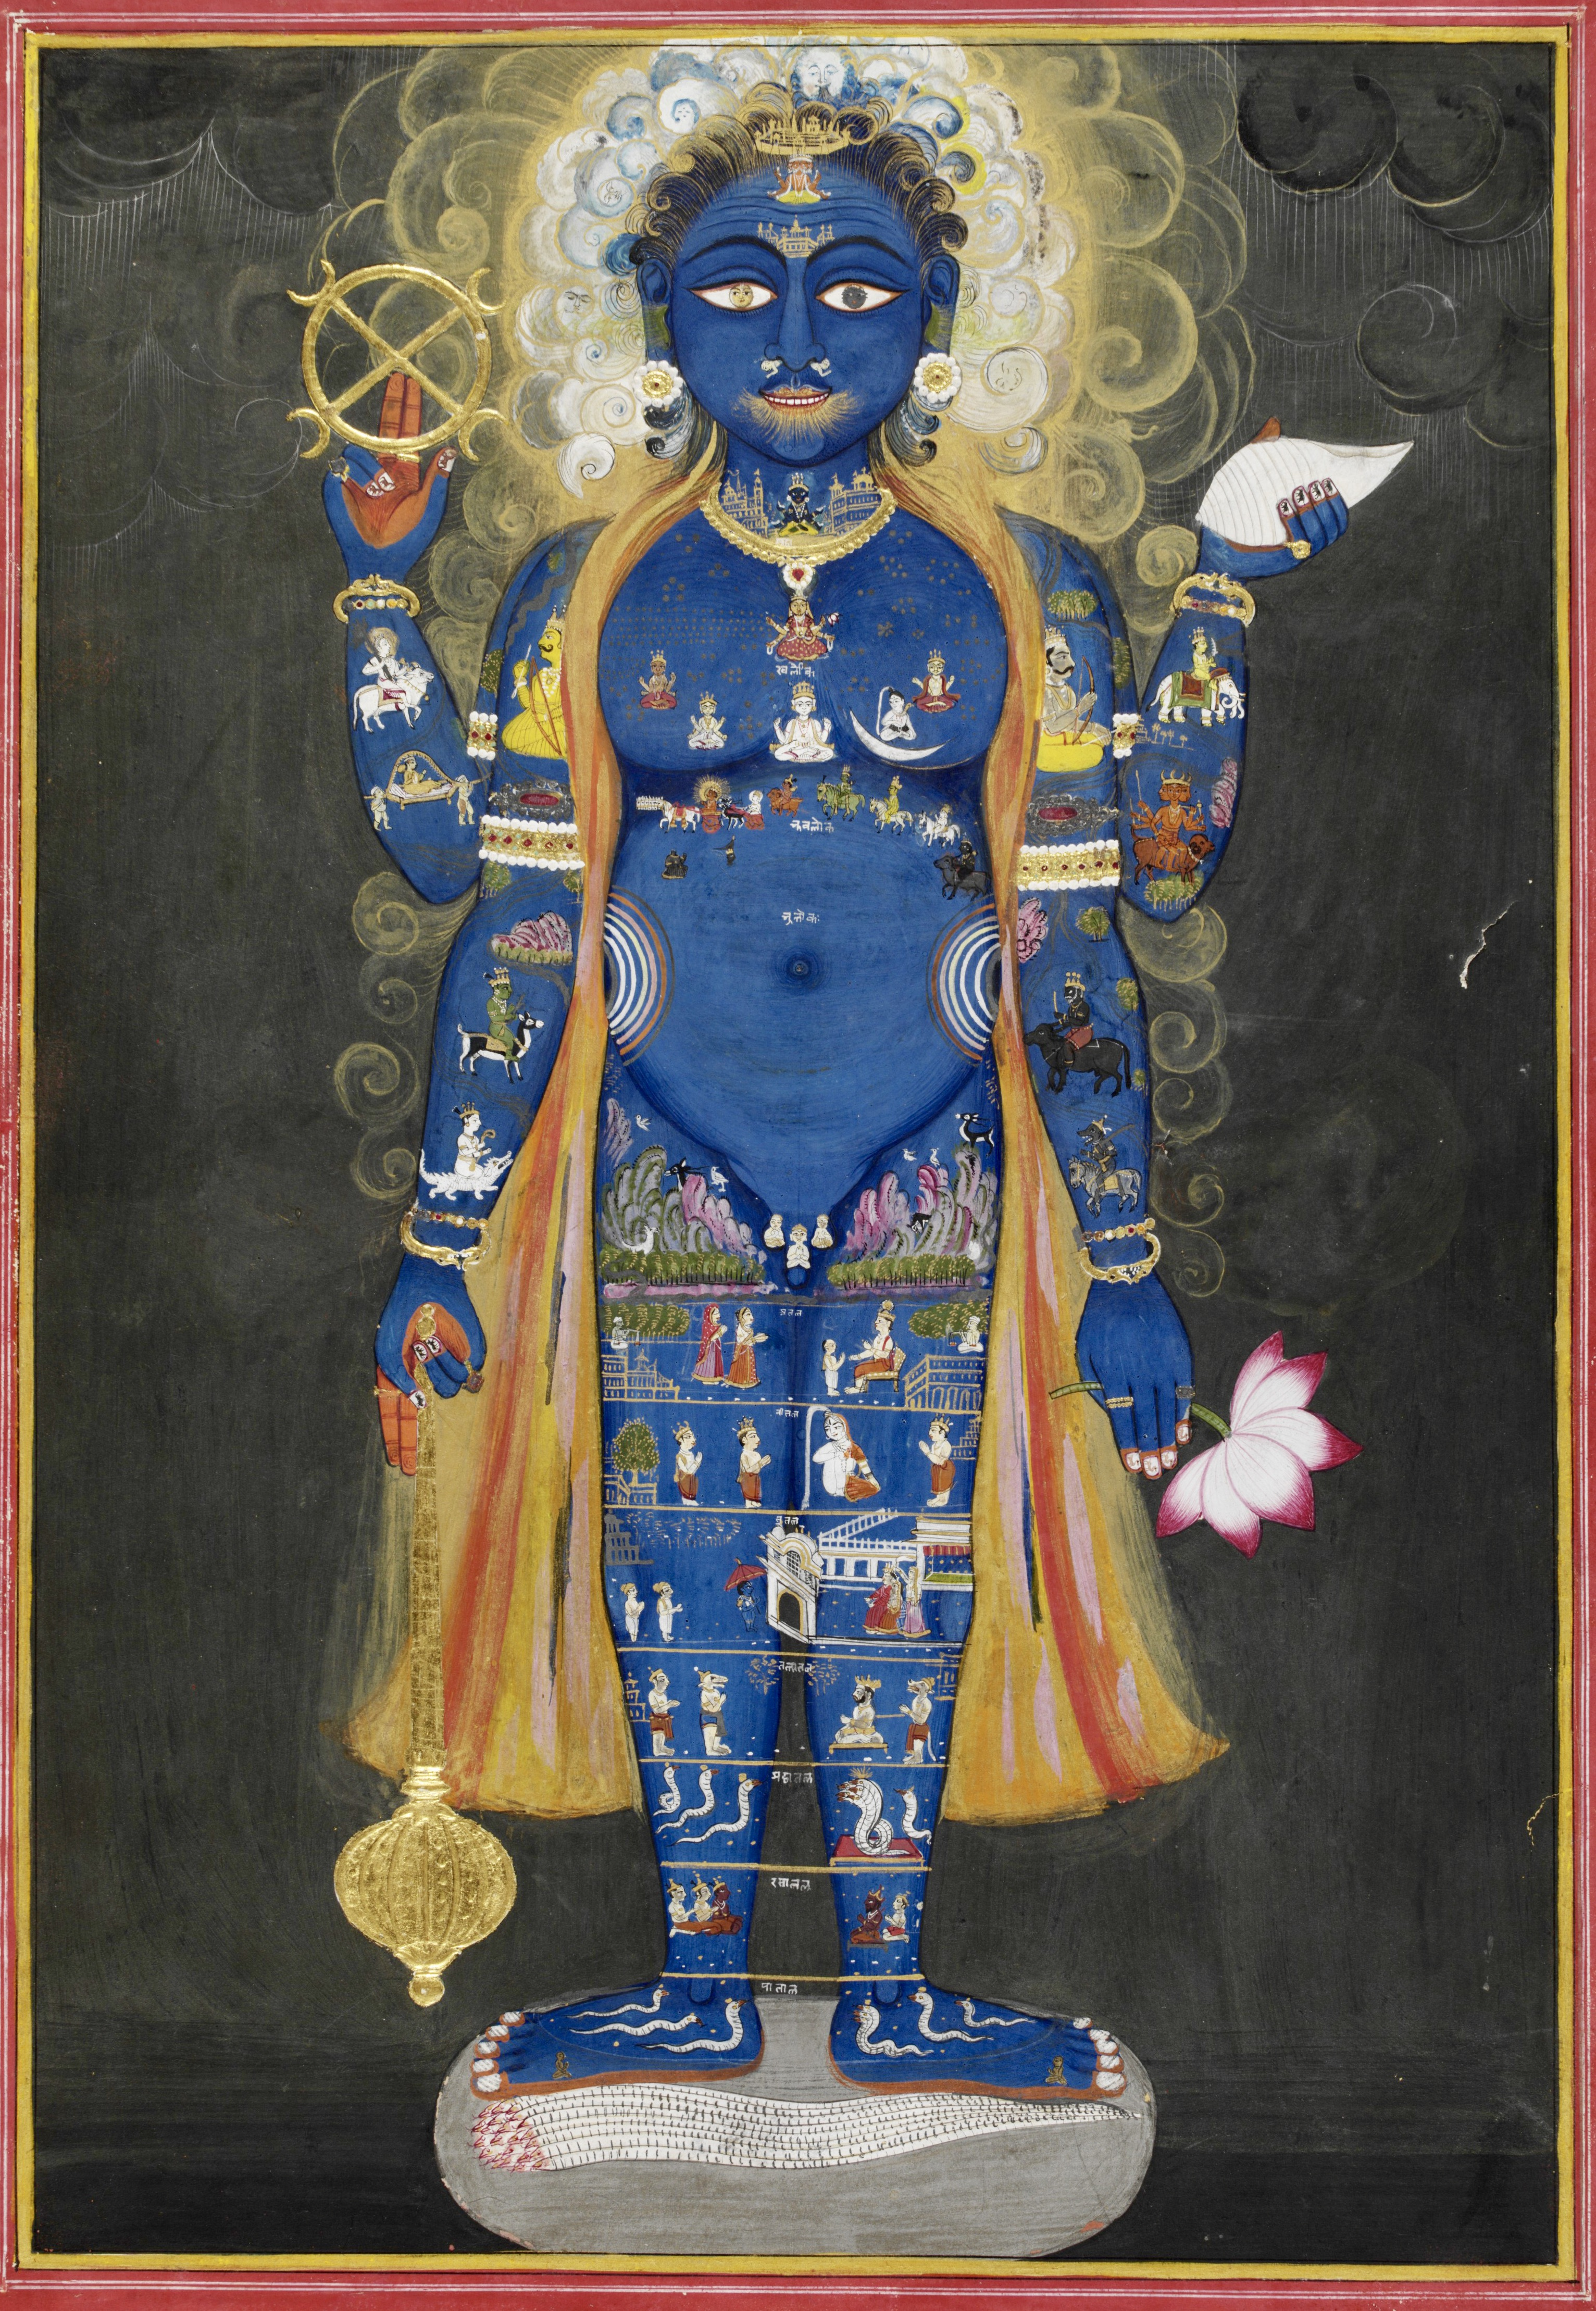
\includegraphics[width=1\textwidth]{pics/Vishnu_Vishvarupa_cropped.jpg}
	\caption{Viṣṇu Viśvarūpa, India, Rajasthan, Jaipur, ca. 1800–1820, Opaque watercolor and gold on paper, 38.5 × 28 cm, Victoria and Albert Museum, London, Given by Mrs. Gerald Clark.}
	\label{fig1}
      \end{figure}
\clearpage
  \begin{figure}[ht]
	\centering
  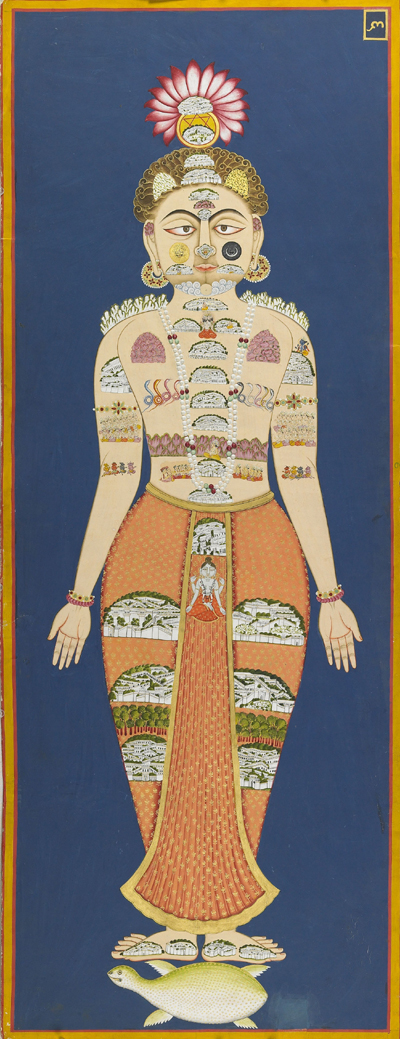
\includegraphics[width=0.5\textwidth]{pics/The_Equivalence_of_Self_and_Universe_(detail),_folio_6_from_the_Siddha_Siddhanta_Paddhati,_(Bulaki),_1824_(Samvat_1881);_122_x_46_cm._Mehrangarh_Museum_Trust..jpg}
	\caption{The Equivalence of Self and Universe (detail), folio 6 from the \textit{Siddhasiddhāntapaddhati} (Bulaki), India, Rajasthan, Jodhpur, 1824 (Samvat 1881), 122 x 46 cm, RJS 2378, Mehragarh Museum Trust.}
	\label{fig2}
      \end{figure}
      % \end{landscape}

      \newpage
      \cleardoublepage
\chapter{Bibliography}
 \label{sec:bibli}
\clearpage
\newpage 
\thispagestyle{empty}
\quad  \addtocounter{page}{-1}

\newrefcontext[sorting=tixel]
\printbibliography[heading=subbibintoc, title=Primary Sources, keyword=primary]

\newrefcontext[sorting=nyt]
\printbibliography[heading=subbibintoc, title=Secondary Literature, keyword=seclit]

\printbibliography[heading=subbibintoc, title=Catalogues, keyword=catalogues]

\printbibliography[heading=subbibintoc, title=Online Sources, keyword=onlinesource]

\end{document}


%%% Local Variables:
%%% mode: latex
%%% TeX-master: t
%%% End:
